\documentclass[a4paper, 11pt]{article}

% packages
\usepackage[utf8]{inputenc}
\usepackage{amsmath}
\usepackage{amsfonts}
\usepackage{array}
\usepackage{booktabs}
\usepackage{chngcntr}
\usepackage{colortbl}
\usepackage{dcolumn}
\usepackage{floatrow}
\usepackage{geometry}
\usepackage{graphicx}
\usepackage{hyperref}
\usepackage{multirow}
\usepackage{natbib}
\usepackage[normalem]{ulem}
\usepackage{ntheorem}
\usepackage{pdflscape}
\usepackage{rotating}
\usepackage{setspace}
\usepackage{subfigure}
\usepackage{tabularx}
\usepackage{threeparttable}
\usepackage[numbib, nottoc, notlot, notlof]{tocbibind}
\usepackage{wrapfig}
\usepackage{xcolor}

% page styling
\geometry{
  a4paper,
  left=1in,
  right=1in,
  bottom=1.2in,
  top=1.2in
}
\pagestyle{plain}
\pagenumbering{arabic}
\linespread{1.5}
\hypersetup{
  colorlinks,
  linkcolor={red!50!black},
  citecolor={blue!50!black},
  urlcolor={blue!80!black}
}
\theoremseparator{:}
\newtheorem{hyp}{Hypothesis}
\counterwithin*{hyp}{section}

\renewcommand{\thefootnote}{\fnsymbol{footnote}}

\title{
	Party Nomination Strategy and its Representational Consequences in Interactive Mixed-Member Majoritarian Systems
	\footnotemark{}
	\footnotetext[1]{This paper was previously entitled and circulated as ``Youth Underrepresentation and Parties' Nomination Strategy in Mixed-Member Electoral Systems". Earlier versions of this paper were presented at the 2024 summer meeting of the Japanese Society for Quantitative Political Science (JSQPS) and the 2024 Annual Meeting of Americal Political Science Association (APSA). I thank Dan Smith for sharing the latest version of his data, and Serika Atsumi, Yuki Atsusaka, Amy Catalinac, Kentaro Fukumoto, Yusaku Horiuchi, Junko Kato, Kenneth McElwain, Mayuko Toba, Masahiro Yamada, Hironao Yoda for their comments.}
}

\author{
	Dai Sasaki
	\thanks{Master's Student, Graduate Schools for Law and Politics, The University of Tokyo. Email: daichansama12@g.ecc.u-tokyo.ac.jp; Website: https://dxxsxsxkx.github.io.}
}

\date{
	First Version: 28 Jun, 2024 \\
	This Version: 6 Dec, 2024 
}

\begin{document}

\maketitle

\renewcommand{\thefootnote}{\arabic{footnote}}
\setcounter{footnote}{0}

\begin{abstract} 
I argue that interactive mixed-member majoritarian systems (interactive MMMs), a variant of mixed member systems where parties can nominate the same candidates in both majoritarian and proportional representation (PR) tiers (dual listing), diminish the representational advantages commonly associated with PR systems. Analyzing comprehensive, candidate-level data of Japan's lower house elections, I show that parties give higher list ranks to senior candidates, incumbents, and dual-listed candidates under the interactive MMM. Furthermore, incumbents are more likely to be dual-listed than non-incumbents. These patterns apply across parties, but are less applicable to situations of intra-party disputes and government transitions, where seniors and incumbents may give their way to newcomers. My analysis suggests that interactive MMMs sustain representational inequalities between groups by reducing the electoral prospects of newcomers and making legislative turnover less frequent.
\end{abstract}

\newpage

\section{Introduction}

Scholars of electoral systems have long recognized that proportional representation (PR) systems help achieve higher levels of minority representation than majoritarian systems \citep{matlandContagionWomenCandidates1996, matlandWomensRepresentationNational1998, meserveGenderIncumbencyParty2020}. The representational advantage of PR over majoritarian systems originate in the voters' evaluation of candidates and parties' response to it. Under (closed) PR, voters generally vote for a list of candidates, not a specific candidate, which means personal votes are less frequent than in majoritarian systems. In such circumstances, parties have incentives to appeal to a broader set of voters by diversifying their lists. PR also falicitates the representation of interests that are geographically scattered \citep{ogradyHowGeographicClustering2024, teelePoliticalGeographyGender2024} or of relatively lower salience \citep{wiedemannRedistributivePoliticsSpatial2024}. As its name suggests, PR improves the proportionality between votes and seats and promotes the representation of benefits that are oft-underrepresented in majoritarian systems. 

Then, how is this representational advantage altered when PR is embedded within an electoral system? This paper focuses on the party nomination strategy in mixed-member majoritarian (MMM) systems, a type of mixed-member (MM) electoral systems \citep{shugartMixedmemberElectoralSystems2003} that combines majoritarian and proportional systems.\footnotemark{} In the other pattern of MM, mixed-member proportional  (MMP) systems, parties' seat shares depend solely on the PR tier and the majoritarian tier decides who gets elected within each party. In contrast, each party's tally in an MMM is the sum of the seats it obtains in the majoritarian and PR tiers. I analyze how parties' nomination strategy in MMMs affects the PR's representational advantage.

\footnotetext{Of the 36 countries that employ MM systems, 27 utilize the MMM variant \citep{catalinacGeographicallyTargetedSpending2021}. These countries span diverse regions and include Andorra, Guinea, Japan, Italy, Libya, Lithuania, Mauritania, Monaco, Nepal, Niger, Pakistan, Panama, the Philippines, Russia, Senegal, Seychelles, Sudan, Taiwan, Tajikistan, Ukraine, Venezuela, Zimbabwe, Hungary, Mexico, Cameroon, and Chad. Some countries recently departed from MMM: for example, Georgia transitioned to a pure-PR following its 2017 constitutional reform, with this change taking effect starting in the 2024 parliamentary election \citep{internationalfoundationforelectoralsystemsElectionsGeorgia20242024}. South Korea adopted a mixed-member proportional (MMP) system for its 2024 National Assembly elections \citep{internationalidea2024SouthKorean2024}.}

This paper shows that institutional arrangements in MMMs could diminish the representational advantage of the PR tier. Specifically, I argue that parties tend to prioritize their senior members and incumbents over others in a variant of MMMs, which I call ``interactive mixed-member systems (interactive MMM)".\footnotemark{} Interactive MMMs allow parties to nominate the same candidates in both majoritarian and PR tiers (dual listing). Even in the PR tier of interactive MMMs, parties still possess incentives to diversify their party lists, because voters vote for a list, not a candidate. However, the following mechanisms would prevail. 

\footnotetext{This terminology helps distinguish the electoral system this paper focuses on from ordinal MMMs or ``parallel systems", where the majoritarian and PR tiers function separately.}

First, the post-election goals of parties incentivize them to maximize the election prospects of senior candidates. Parties are not solely focused on maximizing vote shares but also on electing candidates who can effectively advance their policy goals in parliament, secure key positions within the party, or, for majority-seeking parties, take on government roles. Senior politicians typically possess more political resources than junior politicians, allowing them to perform more effectively in legislative activities and policy-making. In interactive MMMs, parties can provide “insurance tickets” to candidates through dual listing, whereby those losing in the majoritarian tiers may get elected via the PR tier. This mechanism offers senior politicians or incumbents a second chance to be elected.

Another reason parties extensively utilize this mechanism is that dual listing enables parties to monitor candidates' mobilization efforts. Candidates who run solely in the PR tier have less need to cultivate a personal votes and may reduce their campaign efforts by free-riding on others’ work. In contrast, candidates running in both tiers must build personal support in their districts, reducing concerns for the party about their commitment. Furthermore, this mechanism helps parties avoid allegations of favoritism towards specific candidates within their ranks.

This paper analyzes party nomination strategies under interactive MMMs using the case of Japan’s lower house (House of Representatives) elections. Since 1994, Japan’s lower house elections have used an interactive MMM system that permits dual listing. Drawing on data from all candidates who ran in the PR tier from 1994 to 2021, the study examines how parties make their nominations. I conduct the analysis at three levels: aggregate, party, and party-election levels.

The findings reveal that parties tend to favor senior and incumbent candidates when constructing their PR lists, often placing these candidates in higher-ranking positions to improve their chances of being elected. Furthermore, incumbents are shown to have a higher likelihood than non-incumbents of being dual-listed. While not every party demonstrates identical behaviors, each party exhibits some form of preference for senior and incumbent candidates, reflecting the strong incentives created by the system. However, the study also finds that this trend can weaken during periods of internal party conflict or when a governing party transitions to the opposition, leading to a reshuffling of candidates. 

This paper contributes to the relevant literatures in two ways. First, it builds on the extensive body of research examining parties' candidate nomination strategies in the context of electoral systems, particularly PR systems \citep{andrePartyNominationStrategies2017, buisseretPartyNominationStrategies2022, crutzenModelTeamContest2020, dancygierElectoralRulesElectoral2014, hoboltSelectionSanctioningEuropean2011, nemotoLocalismCoordinationThree2013}. Prior studies have demonstrated that under closed-list or flexible-list PR, the ranking of candidates on party lists reflects the party’s prioritization of those candidates. These studies consistently suggest that parties place “stronger” candidates—defined by factors such as cognitive ability, education, or the ability to attract preference votes—at the top of their lists \citep{buisseretPartyNominationStrategies2022, coxMoralHazardElectoral2021}. However, the question of how candidate nomination strategies might change when the proportional formula is embedded within a mixed-member electoral system, rather than used independently, has received little attention. Although this paper does not address all aspects of party nomination strategies under MMM broadly, it provides a meaningful contribution by identifying specific patterns of candidate prioritization under particular institutional arrangements. 

Second, and most importantly, this paper demonstrates that the representative advantages typically associated with PR systems can be undermined under interactive MMMs. In this system, parties are incentivized to provide insurance to senior and incumbent candidates through dual candidacy. This practice, while strategic for ensuring the election of experienced candidates, inadvertently restricts the entry of new candidates. Consequently, the nomination strategies of parties under interactive MMMs may delay or prevent the inclusion of underrepresented groups who are already disadvantaged at the time the system is introduced. To illustrate this, the paper uses the example of youth underrepresentation in Japan. While PR systems are often praised for their ability to promote the representation of minorities, cross-national comparisons have shown that PR systems generally result in a higher proportion of younger legislators compared to majoritarian systems \citep{stockemerAgeRepresentationParliaments2018, stockemerAgeInequalitiesPolitical2023}. However, in mixed-member systems, if the institutional design is not carefully considered, the inherent representational benefits of PR can be diminished or entirely lost.

This paper proceeds as follows. Section \ref{sec: the} discusses the theoretical backgrounds of the research, presents the main arguments, and formulate hypotheses. It discusses how parties would render their nomination strategies where the two tiers are institutionally interacted. I also outline Japan's mixed-member system with a focus on dual listing. Section \ref{sec: emp} presents the data and empirical strategies. Section {sec: res} shows the results of the analysis. It presents aggregate-level and party-specific evidence, as well as election- and party-specific analysis. Section \ref{sec: dis} discusses the implication of the results, focusing on legislative turnover and representation. 

\section{Theory} \label{sec: the}

\subsection{Theoretical Expectations}

It remains unclear how party nomination strategies and patterns uncover in mixed-member systems, in contrast to ``pure" electoral systems. MM systems have often been regarded to deliver ``the best of both worlds", that is, majoritarian and PR \citep{shugartMixedmemberElectoralSystems2003, hiranoPolicyPositionsMixed2011}. This perception stems from the theoretical argument that MM helps avoid the extreme outcomes associated with pure systems on both inter-party and intra-party dimensions. On the inter-party dimension, MM combines the features of majoritarian systems, which favor two-party dominance, and PR systems, which facilitate the representation of smaller parties. As a result, MM is thought to mitigate the vote-seat disproportionality inherent in majoritarian systems. For example, under a mixed system, it is expected to be less likely for a party to secure a legislative majority without achieving an absolute majority of the vote, as frequently observed under pure majoritarian systems. On the intra-party dimension, mixed systems are believed to balance competing incentives by preserving and fostering ties between voters and candidates through the nominal tier while simultaneously enhancing party cohesion through the list tier.

However, scholars have noted that mixed systems do not necessarily occupy a middle ground between the two pure systems in all respects. In fact, the interaction between the two tiers within mixed systems can create what is referred to as a “contamination effect,” where one tier influences the dynamics of the other. Much of the existing research on mixed systems has focused on the implications of these contamination effects for party systems \citep{bawnComparativeTheoryElectoral2003, coxInteractionEffectsMixedMember2002, ferraraMixedElectoralSystems2005, herronContaminationEffectsNumber2001, nishikawaMixedElectoralRules2004, moserMixedElectoralSystems2004}. Key areas of inquiry include how the actual number of parties or candidates deviates from the theoretical predictions of Duverger’s law, the nature of the relationship between vote shares and seat shares, and the responsiveness of candidates to different types of electoral incentives.

In contrast to previous studies, however, this article is concerned with how MMM systems are positioned relative to pure systems in terms of candidate nomination strategies and representativeness. Specifically, it examines whether the institutional features of MMM systems lead to patterns that align more closely with majoritarian, pure PR, or something distinct. To the author’s knowledge, few studies have directly addressed these questions with regard to MMMs. While related research exists, it often focuses on other mixed systems, such as MMP systems, or on broader aspects of electoral outcomes rather than nomination strategies or representativeness. For instance, \citet{fortin-rittbergerGenderEqualBundestagImpact2013} found that women’s descriptive representation improved under Germany’s MMP system. However, their findings highlighted the role of voluntary quotas adopted by political parties, rather than the electoral system itself, in improving gender representation.

This paper argues that the institutional configuration of MMMs creates incentives for parties to favor senior candidates in the PR tier. Specifically, these incentives arise under interactive MMM systems, which allow dual listing—nominating the same candidate in both the majoritarian and proportional tiers. While dual listing is commonly associated with MMPs, such as in Germany and New Zealand \citep{konoDualCandidacyRemedy2020, electoralcommisionofnewzealandNewZealandsElectoral2014}, it is also utilized in MMM systems as in Japan, Hungary, Italy, and Lithuania \citep{pappDualCandidacySource2021, lemondeHowDoesItalian2022, thecentralelectoralcommissionoftherepublicoflithuaniaElectionsReferendum2024}. This paper contends that the use of dual listing in interactive MMM plays a key role in shaping party nomination strategies, particularly by encouraging the prioritization of experienced candidates.

Existing research provides insights into how dual listing operates in mixed systems, though much of this work has focused on its effects rather than its implications for candidate selection. For example, \citet{mckeanJapansNewElectoral2000} demonstrate that dual listing can reduce the ratio of candidates to available seats, a pattern that reflects the strategic consolidation of party resources. Meanwhile, \citet{kraussReverseContaminationBurning2012} highlight that parties and candidates can use PR list rankings to send signals to voters, encouraging strategic voting in the majoritarian tier for those with lower list ranks in the PR tier. These studies underscore the multifaceted role that dual listing plays in shaping electoral dynamics, but they have not fully examined how this mechanism influences the representational quality of proportional tiers within MMM systems. By focusing on this gap, the present study aims to shed light on the broader implications of interactive MMM for candidate nomination strategies and the diversity of legislative representation.

How does dual listing influence party nomination strategies? This paper argues that the allowance of dual listing in interactive MMMs incentivizes parties to provide “insurance tickets” to senior politicians. For political parties, it is crucial not only to maximize the number of seats they win but also to determine which candidates fill those seats. This dual priority stems from the nature of political parties, which function not just as vote-gathering mechanisms during elections but also as organizations with post-election legislative and governance goals \citep{matakosElectoralInstitutionsIntraparty2024}. In this context, parties face two competing incentives: on one hand, they aim to continue electing senior candidates who can occupy leadership roles within the party or government; on the other hand, they must foster the election of new candidates to groom future senior members. Given that parties estimate the number of seats they can realistically win, their nomination strategy can be seen as solving an optimization problem under the constraint of attainable seats.

As policy-driven entities, parties rank candidates based on seniority, as senior members typically possess critical resources for policymaking. These resources include expertise in drafting policies, legislative process knowledge, negotiation skills with other parties, coordination with bureaucracies, and connections with stakeholders. Generally, politicians acquire these resources through experience, creating a positive correlation between tenure and resource accumulation. A similar dynamic exists between incumbent and non-incumbent candidates. When possible, parties reflect these priorities in their nomination strategies \citep[p.1085]{reedNominationProcessJapans1995}. Dual listing provides an avenue for parties to act on these incentives. By nominating senior politicians or incumbents on both tiers, parties can offer them an “insurance ticket.”

However, if parties merely valued senior candidates, they could simply place them at the top of PR lists without using dual listing. In PR nominations, parties prioritize candidates who can attract substantial party votes. While nominating nationally recognized celebrities is one approach, their competency may be uncertain. A more reliable option is to nominate veteran politicians with proven abilities and high name recognition \citep{reedNominationProcessJapans1995}. Nevertheless, the use of dual listing is driven by the institutional features of mixed-member systems.

In MMMs, winning in single-member districts (SMDs) is critical for majority-seeking parties \citep{bawnComparativeTheoryElectoral2003, catalinacGeographicallyTargetedSpending2021}, but candidates capable of succeeding in SMDs are scarce. In interactive MMM, parties use dual listing to provide a “second chance” to promising SMD candidates, thereby managing long-term priorities. This approach reassures candidates by offering a backup plan, ensuring that even if they lose in the SMD, they can still win via the PR tier and maintain their ties with voters as incumbents. At the same time, parties ensure these candidates remain motivated by requiring their SMD candidacy \citep{bawnComparativeTheoryElectoral2003}. This method avoids accusations of favoritism while still strategically managing resources. For example, parties can nominate candidates for safe PR seats while deploying them as challengers in competitive SMDs \citep{reedNominationProcessJapans1995}. However, this strategy risks perceptions of nepotism among other party members and does not guarantee that the candidate will excel in their legislative role.

For certain candidates, such as those with unassailable reputations, established SMD performance, or those nearing retirement and preparing successors, dual listing’s “carrot and stick” approach may be unnecessary. These candidates can be directly placed in PR seats or contested freely in SMDs without additional oversight. \footnotemark{}

\footnotetext{In Japan, former prime ministers Yasuhiro Nakasone and Kiichi Miyazawa were once granted the top position on the PR list \citep{theasahishimbunNakasoneMiyazawaRyou2006}.}

When dual listing is allowed, parties face two key options for PR nominations: providing insurance to existing SMD candidates or nominating entirely new candidates. These options are, to some extent, mutually exclusive. Party resources, such as campaign funding and organizational support, are finite, and the number of candidates parties can field simultaneously is limited. Parties also align their nominations with the expected number of seats they believe they can win, making excessive over-nomination rare. Consequently, when parties use dual listing to enhance the electoral prospects of existing members, they tend to nominate fewer new candidates. Even when new candidates are nominated, their chances of election are not necessarily high. In closed-list PR systems, a candidate’s position on the list directly correlates with their likelihood of election: the higher the rank, the greater the chances. As long as parties prioritize senior or incumbent candidates, new candidates are likely to be placed in lower, less winnable positions on the list.

Based on the above discussion, five hypotheses are proposed: 

\begin{hyp}[H\ref{hyp:first}] \label{hyp:first}
Senior candidates (i.e., those with more terms in office) are assigned higher positions on the proportional representation (PR) list compared to less senior candidates.
\end{hyp}

\begin{hyp}[H\ref{hyp:second}] \label{hyp:second}
Incumbents are assigned higher positions on the PR list compared to non-incumbents.
\end{hyp}

\begin{hyp}[H\ref{hyp:third}] \label{hyp:third}
The more senior a candidate is, the more likely they are to be dual-listed.
\end{hyp}

\begin{hyp}[H\ref{hyp:fourth}] \label{hyp:fourth}
Incumbents are more likely to be dual-listed than non-incumbents.
\end{hyp}

\begin{hyp}[H\ref{hyp:fifth}] \label{hyp:fifth}
Dual-listed candidates are assigned higher positions on the PR list compared to non-dual-listed candidates.
\end{hyp}

These hypotheses are expected to hold across all political parties. For large parties, which are likely to secure numerous seats in each election and have a strong incentive to win government, there is a significant motivation to elect candidates capable of serving in cabinet positions. Large parties often have a wealth of experienced members and internal practices that allocate roles based on seniority, reinforcing their incentive to prioritize senior and incumbent candidates for dual listing and higher PR positions.

For smaller parties, while they may have an incentive to use PR lists to bring in younger politicians, they are also likely to utilize dual listing to ensure the election of their core members. Given the uncertainty of winning in single-member districts (SMDs), smaller parties often rely on their PR vote share to secure a stable number of seats. In MMMs, smaller parties may also exchange votes across tiers with larger parties \citep{catalinacGeographicallyTargetedSpending2021}. For example, smaller parties may support larger party candidates in SMDs in exchange for proportional votes. Under these circumstances, smaller parties have an incentive to provide insurance to senior and incumbent candidates by prioritizing them on PR lists or dual-listing them.

However, there are conditions under which Hypotheses 1 and 3 may be weaker: First, the incentive to insure senior candidates diminishes when a party loses its majority and falls out of government, as the need to fill key government roles decreases. Second, if a party enters an election amid factional disputes, the dominant faction may have an incentive to sideline members of opposing factions rather than granting them insurance through high PR positions or dual listing. 

\subsection{Case: Japan's Mixed-Member Majoritarian System}

This paper examines the above hypotheses using data from Japan’s House of Representatives elections under its MMM system. In 1994, Japan underwent electoral reform, adopting a MMM system that combines SNTV-SMD and PR tiers. When a new electoral system is introduced, political actors gradually adapt to its rules and incentives. Therefore, to accurately evaluate the behavioral patterns and incentive structures under a given system, it is crucial to analyze it after sufficient time has elapsed for adaptation. In this respect, Japan’s MMM system, implemented nearly 30 years ago, provides a suitable case for examining the long-term incentives created by this institutional framework. Furthermore, dual listing is widely utilized in Japan, garnering significant public and media attention. Figure \ref{fig:dual} illustrates the proportion of candidates elected via the PR tier who were dual-listed in each House of Representatives election. Since 2000, more than half of all PR-elected candidates have consistently been dual-listed. This trend highlights the strategic importance of dual listing under Japan’s MMM system, providing a rich context for analyzing how it shapes candidate selection and ranking strategies.

\begin{figure}[!htbp]
	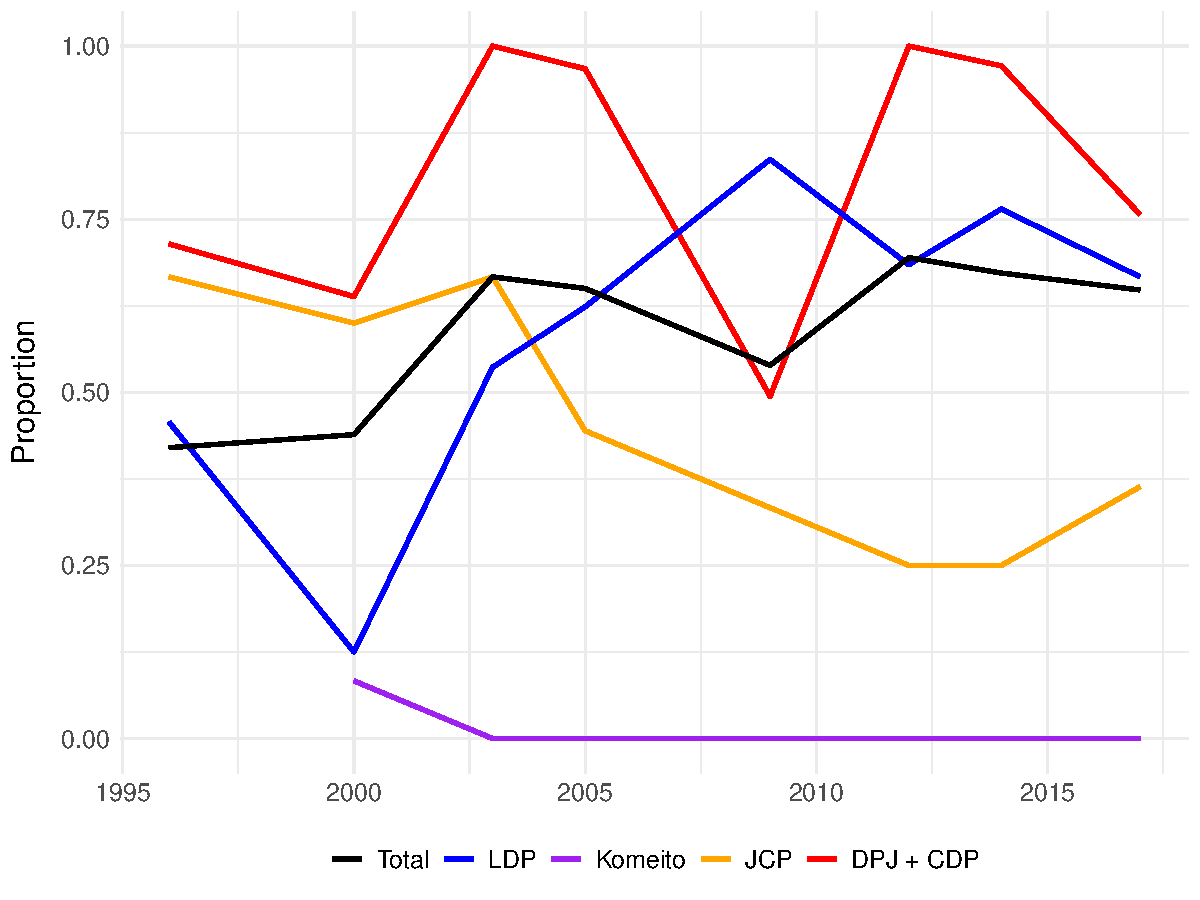
\includegraphics[width = 0.9\textwidth]{../figure/paper/dual_nomination.pdf}
	\caption{Share of Dual-Listed Candidates among PR Winners}
	\label{fig:dual}
\end{figure}

MPs who secure a seat through dual listing (i.e., losing in the SMD but winning in the PR) are often derisively termed "zombie MPs." The prevalence of this "resurrection" pattern is frequently highlighted in media coverage, attesting to its common occurrence. Moreover, comprehensive candidate-level data for Japan \citep{reedReedSmithJapaneseHouse2017} enables detailed analysis of party candidate nomination patterns. To the best of our knowledge, no other country using an MMM system possesses such granular candidate data. These factors make Japan an exceptionally suitable case for analyzing candidate nomination patterns under an interactive MMM.

Prior to the electoral reform, Japan employed an SNTV-MMD system. A key feature of this system was the possibility of multiple candidates from the same party winning in a single MMD. This necessitated candidates to differentiate themselves from their party colleagues to secure personal votes, often leading to political corruption. The prevalence of such corruption was a catalyst for electoral reform.

The primary objective of electoral reform was to shift elections from a candidate-centered to a policy- and party-centered focus. The Eighth Electoral System Council, established in June 1989, submitted a reform proposal in April 1990. This proposal emphasized increasing the likelihood of government change and advocated for the adoption of a mixed-member majoritarian (MMM) system with a strong SMD component \citep{theasahishimbunShuuinNiShousenkyoku1990, yoshidaChusenkyokuseiKaraShosenkyokuhireidaihyou2018}. While the council also considered MMP \citep{theasahishimbunSenkyoseidoshinNoGijiroku1991}, and some parties (especially Komeito and Socialist Party) proposed similar systems, these were not adopted. Although the Kaifu Cabinet, which received the council's proposal, failed to implement the draft, the subsequent Hosokawa Cabinet enacted a nearly identical reform.

The new system combined SMD (SNTV-SSD) and PR tiers. Under this system, voters cast two ballots: one for an SMD candidate and another for a party list in the PR block. Personal votes could not be cast in the PR block (closed-list). The number of seats a party won was the sum of its SMD and PR seats. SMD seats were determined using SNTV, while PR seats were allocated to parties within each block using the d'Hondt method, and then distributed among candidates within each party.

Japan's MMM is an interactive system that permits dual listing \citep{pekkanenElectoralIncentivesMixedMember2006, reedJapaneseElectoralSystems2020}. Parties can nominate candidates for both the SMD and PR. Additionally, parties can assign the same list position to multiple dual candidates. Table \ref{tab:listStructure} presents possible list composition patterns in Japan's MMM. Parties can choose not to use dual listing and simply rank candidates from top to bottom (List A). Alternatively, they can dual list multiple candidates and assign the same rank to some (List B) or all (List C). As List B shows, it is not necessary to place all dual candidates at the top. It is also possible to create multiple strata among dual candidates (List D). However, it is not permissible to assign the same rank to candidates who are not dual listed (List E).

% created manually
\begin{table}[!htbp]
\centering
\begin{threeparttable}
\begin{tabular}{cccccccccc}
\toprule
\multicolumn{8}{c}{Valid} & \multicolumn{2}{c}{Invalid} \\
\cmidrule(lr){1-8} \cmidrule(lr){9-10}
\multicolumn{2}{c}{List A} & \multicolumn{2}{c}{List B} & \multicolumn{2}{c}{List C} & \multicolumn{2}{c}{List D} & \multicolumn{2}{c}{List E} \\
\cmidrule(lr){1-2} \cmidrule(lr){3-4} \cmidrule(lr){5-6} \cmidrule(lr){7-8} \cmidrule(lr){9-10}
Rank & Dual & Rank & Dual & Rank & Dual & Rank & Dual & Rank & Dual \\
\cmidrule(lr){1-2} \cmidrule(lr){3-4} \cmidrule(lr){5-6} \cmidrule(lr){7-8} \cmidrule(lr){9-10}
1 & - & 1 & - & 1 & \checkmark & 1 & \checkmark & 1 & - \\
2 & - & 2 & \checkmark & 1 & \checkmark & 1 & \checkmark & 1 & - \\
3 & - & 2 & \checkmark & 1 & \checkmark & 3 & \checkmark & 3 & - \\
4 & - & 2 & \checkmark & 1 & \checkmark & 3 & \checkmark & 4 & \checkmark \\
5 & - & 2 & \checkmark & 5 & - & 5 & - & 5 & \checkmark \\
6 & - & 6 & \checkmark & 6 & - & 6 & - & 6 & - \\
7 & - & 7 & \checkmark & 7 & - & 7 & - & 7 & - \\
8 & - & 8 & \checkmark & 8 & - & 8 & - & 8 & - \\
\bottomrule
\end{tabular}
\begin{tablenotes}[flushleft]
  \scriptsize{
    \item \textit{Note.} This table presents five hypothetical party lists that may be submitted in the PR tier of Japan's mixed member majoritarian system. Dual-listed candidates are denoted by \checkmark. Lists A, B, C, and D are all valid. List E is invalid, as pure-PR candidates cannot be ranked equal. 
  }
\end{tablenotes}
\end{threeparttable}
\caption{Valid and Invalid List Structures in Japan's Interactive MMM system}
\label{tab:listStructure}
\end{table}



















The final list order, which determines the allocation of seats within a party, is adjusted based on the SMD election results. First, SMD winners among dual candidates are removed from the list. Second, candidates with the same rank are sorted based on their performances in the SMD tier.\footnotemark{} The final seat allocation within the party is then based on this revised list order.

\footnotetext{Technically, candidates are reranked according to what is called ``close-loss rate". Let $i$ be a SMD-losing dual-listed candidate in the district $d$. Candidate $i$'s close loss rate, $\text{Loss}_{i}$, is calculated as 
  \[
    \text{Loss}_{i} = \frac{\text{Vote}_i}{\text{max}(\text{Vote}_d)}, 
  \]
\noindent where $\text{max}(\text{Vote}_d)$ denotes the largest number of votes obtained in the district $d$ (i.e., that of the winner). 
}

The exact process by which this system was included in the new electoral system is unclear. The Eighth Electoral System Council's proposal already included this provision \citep{yoshidaChusenkyokuseiKaraShosenkyokuhireidaihyou2018}. However, the council's minutes are not publicly available, making it impossible to determine who proposed the inclusion of this provision or at what stage \citep{theasahishimbunSenkyoseidoshinNoGijiroku1991}.

\section{Data and Method} \label{sec: emp}

To test the hypotheses, I use the Japanese House of Representatives Elections Dataset (JHRED; \citet{reedReedSmithJapaneseHouse2017}). Specifically, I analyze the nomination patterns of candidates running in the PR tier of the post-reform general election between 1996 and 2021. This criterion leaves 7,754 candidates across nine elections (2000, 2003, 2005, 2009, 2012, 2014, 2017, and 2021). Table \ref{tab:stats} in the appendix presents candidate-level summary statistics. 

I estimate a series of logistic and negative binomial models. For Hypotheses \ref{hyp:first}, \ref{hyp:second}, and \ref{hyp:fifth}, the dependent variable is the list rank of candidates. I estimate negative binomial models, as the rank of a candidate in the PR list can be treated as count data, representing how many candidates are ranked higher than the given candidate. For Hypotheses \ref{hyp:third} and \ref{hyp:fourth}, the dependent variable is the dual listing dummy that takes a value of one for dual-listed candidates. Logit models are estimated for this variable. I also use estimate logistic models where the dependent variable is the tie dummy, which equals unity for candidates that are dual-listed and are ranked the same as other candidates (c.f., Lists B, C, and D in Table \ref{tab:listStructure}). 

In addition to the above covariates, I also include a tie dummy, where a value of 1 is assigned to candidates who are dual-listed and are ranked the same as other candidates, to distinguish patterns among dual-listed candidates. This dummy variable is interacted with the dual listing dummy, the number of past wins, and incumbent dummy, where applicable. 

I include a number of covariates in the models, including a female dummy, district magnitude, and two-way fixed effects for election year and party. I control for candidates' gender because parties have incentives to give female candidates favorable positions in PR lists to appeal to a broader set of voters \citep{salmondProportionalRepresentationFemale2006, chiruValueLegislativeElectoral2017}. I also account for block magnitudes, as the length of a list depends on the maximum number of candidates elected. Magnitudes vary across time and region: see Table \ref{tab:distM} in the appendix for details. Party FE accounts for different nomination patterns among parties. For example, \citet{fujimuraShousenkyokuHireidaihyouHeiritsusei2012} finds different patterns in allocating the parties' important positions for the dominant Liberal Democratic Party (LDP) and Democratic Party of Japan (DPJ), two largest parties in the country at the time. Given party-level variations in the candidate evaluation, it is reasonable to assume party-specific patterns of candidate nomination. For a similar reason, standard errors are clustered at the party level. I also control for the tie dummy mentioned above, along with interaction terms between the tie dummy and the dual listing dummy, number of past wins, and incumbent dummy, where applicable. I intend to account for differential nomination patterns for those who have ties on the party list and those who do not. 

In party-specific and election year-specific analyses, I exclude corresponding fixed effects from the models. In the party-specific analysis, I analyze the four parties or party groups: LDP, DPJ and its successor Constitutional Democratic Party (CDP), Komeito, and Japan Communist Party (JCP). In the party/election-level analysis, l focus on the Liberal Democratic Party in the years 2005 and 2012.

\section{Result} \label{sec: res}

\subsection{Aggregate-Level Analysis}

% TODO: write


\begin{table}
\begin{center}
\begin{tabular}{l c c c c c c c c c c}
\hline
 & \multicolumn{4}{c}{List Rank} & \multicolumn{3}{c}{Dual Listing} & \multicolumn{3}{c}{Dual Listing (Tie)} \\
\cline{2-5} \cline{6-8} \cline{9-11}
 & Model 1 & Model 2 & Model 3 & Model 4 & Model 5 & Model 6 & Model 7 & Model 8 & Model 9 & Model 10 \\
\hline
Total Wins         & $-0.15^{***}$ &               &               & $-0.10^{***}$ & $0.16^{***}$ &              & $-0.00$      & $0.14^{***}$ &              & $0.00$        \\
                   & $(0.01)$      &               &               & $(0.02)$      & $(0.04)$     &              & $(0.02)$     & $(0.04)$     &              & $(0.02)$      \\
Incumbency         &               & $-1.02^{***}$ &               & $-0.74^{***}$ &              & $1.33^{***}$ & $1.33^{***}$ &              & $1.16^{***}$ & $1.13^{***}$  \\
                   &               & $(0.12)$      &               & $(0.11)$      &              & $(0.28)$     & $(0.28)$     &              & $(0.32)$     & $(0.31)$      \\
Dual Listing       &               &               & $-1.82^{***}$ & $-0.93^{***}$ &              &              &              &              &              &               \\
                   &               &               & $(0.25)$      & $(0.27)$      &              &              &              &              &              &               \\
Tie                &               &               &               & $-1.92^{*}$   &              &              &              &              &              &               \\
                   &               &               &               & $(0.86)$      &              &              &              &              &              &               \\
Female             &               &               &               & $-0.07$       &              &              & $-0.24^{*}$  &              &              & $-0.40^{***}$ \\
                   &               &               &               & $(0.04)$      &              &              & $(0.12)$     &              &              & $(0.11)$      \\
Block Magnitude    &               &               &               & $0.02^{***}$  &              &              & $0.04^{***}$ &              &              & $0.04^{***}$  \\
                   &               &               &               & $(0.01)$      &              &              & $(0.01)$     &              &              & $(0.01)$      \\
Total Wins x Tie   &               &               &               & $0.10^{***}$  &              &              &              &              &              &               \\
                   &               &               &               & $(0.02)$      &              &              &              &              &              &               \\
Tie x Incumbency   &               &               &               & $0.49^{**}$   &              &              &              &              &              &               \\
                   &               &               &               & $(0.18)$      &              &              &              &              &              &               \\
Tie x Dual Listing &               &               &               & $0.84$        &              &              &              &              &              &               \\
                   &               &               &               & $(0.91)$      &              &              &              &              &              &               \\
\hline
Year FE            & Yes           & Yes           & Yes           & Yes           & Yes          & Yes          & Yes          & Yes          & Yes          & Yes           \\
Party FE           & Yes           & Yes           & Yes           & Yes           & Yes          & Yes          & Yes          & Yes          & Yes          & Yes           \\
AIC                & $37167.39$    & $36446.03$    & $33098.42$    & $31652.57$    & $5886.23$    & $5697.89$    & $5629.09$    & $5949.29$    & $5803.79$    & $5729.36$     \\
Log Likelihood     & $-18536.69$   & $-18176.02$   & $-16502.21$   & $-15771.28$   & $-2897.12$   & $-2802.94$   & $-2765.54$   & $-2928.64$   & $-2855.90$   & $-2815.68$    \\
Num. obs.          & $7754$        & $7754$        & $7754$        & $7754$        & $7754$       & $7754$       & $7754$       & $7754$       & $7754$       & $7754$        \\
\hline
\multicolumn{11}{l}{\scriptsize{\item $^{***}p<0.001$; $^{**}p<0.01$; $^{*}p<0.05$. Standard errors clustered at the party level in parentheses.
\item Dependent variable: candidate $i$'s list rank (columns 1-4) dual listing status (columns 5-7), and whether the candidate has a tie on the list (columns 8-10).
\item Estimated models: negatige binomial (columns 1-4) and logit (columns 5-10).}}
\end{tabular}
\caption{Regression Results}
\label{tab:regression_results}
\end{center}
\end{table}


\begin{figure}[!htbp]
	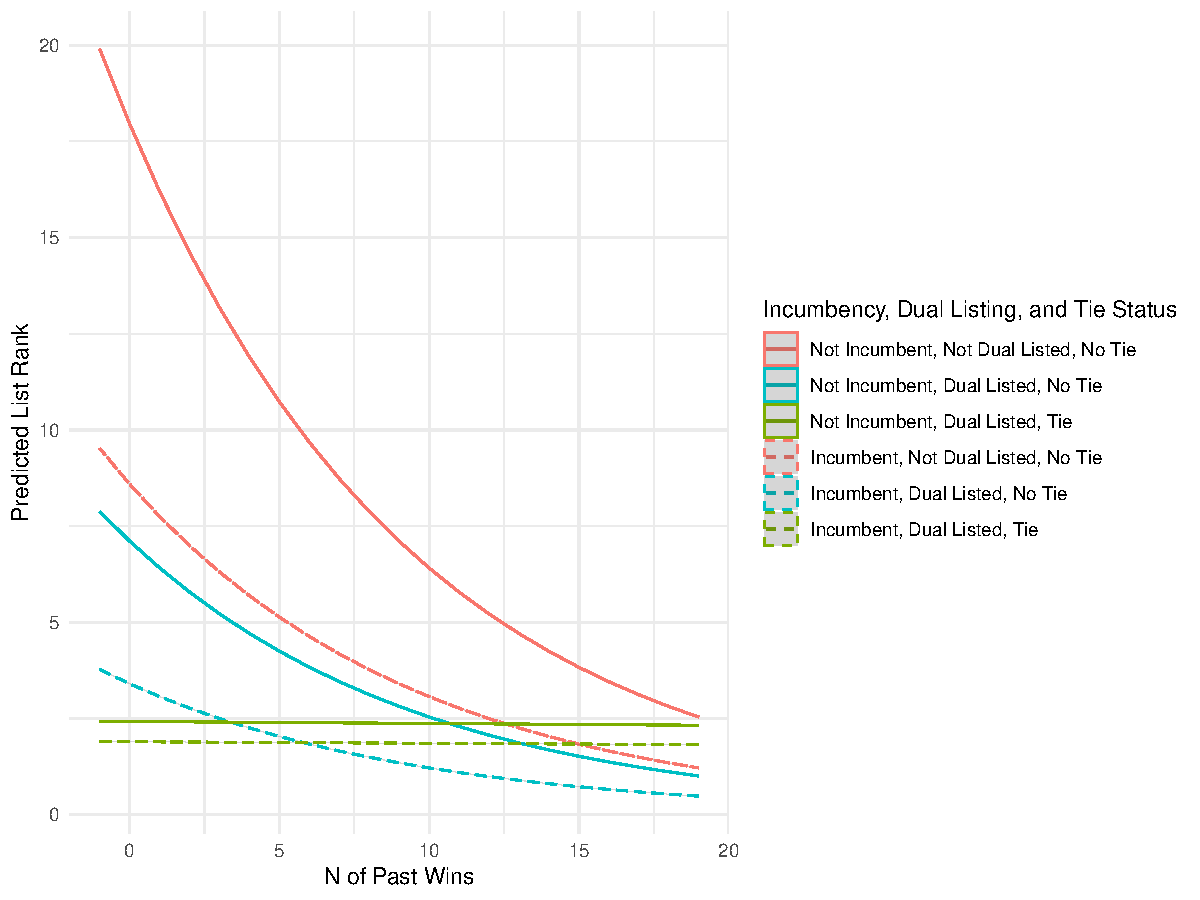
\includegraphics[width = 0.9\textwidth]{../figure/paper/marginal_effects_rank.pdf}
	\caption{Marginal Effects of Seniority, Incumbency, Dual Listing, and Tie Status on List Rank}
	\label{fig:marginal_rank}
\end{figure}

\begin{figure}[!htbp]
	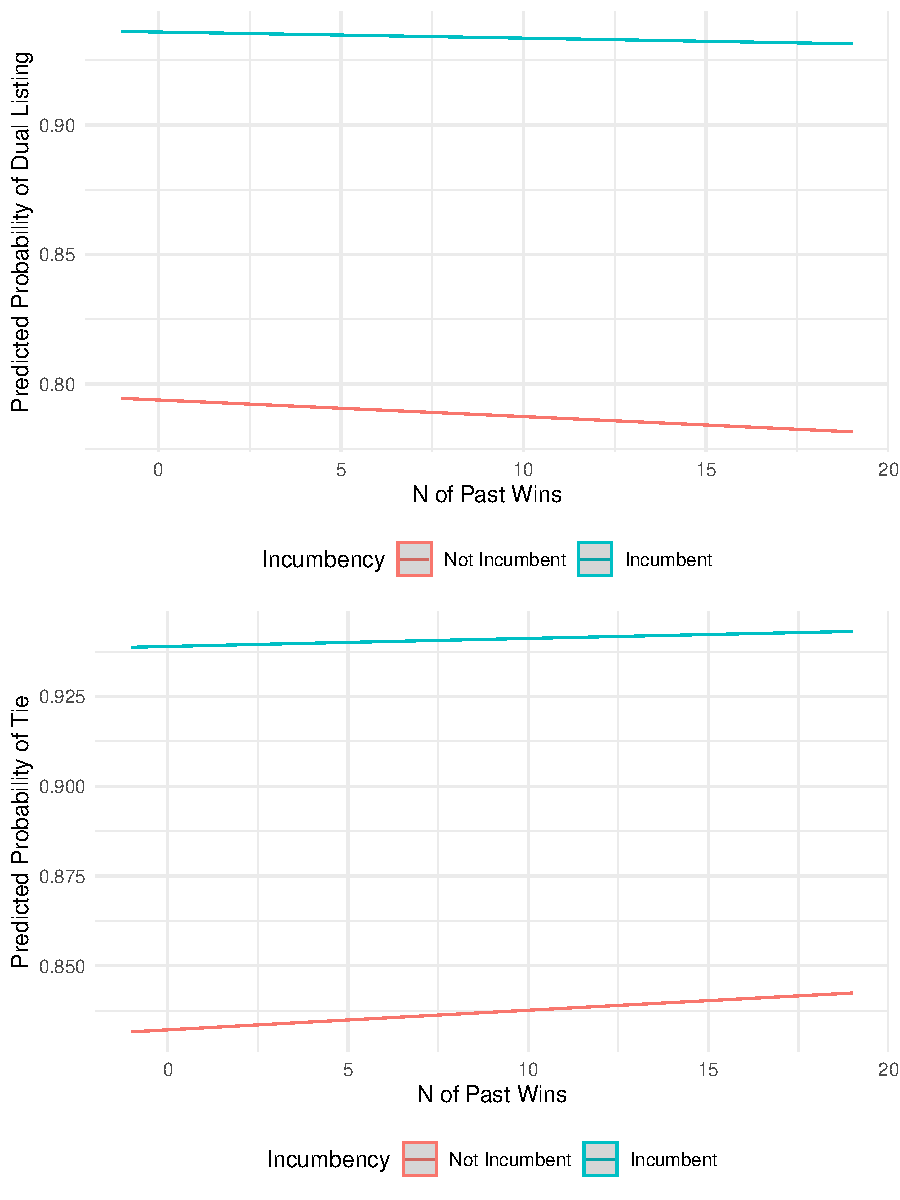
\includegraphics[width = 0.9\textwidth]{../figure/paper/marginal_effects_dual_tie.pdf}
	\caption{Marginal Effects of Seniority and Incumbency on Dual Listing}
	\label{fig:marginal_dual}
\end{figure}


\subsection{Party-Specific Analysis}

% TODO: write


\begin{table}[!htbp]
\begin{center}
\scalebox{0.6}{
\begin{threeparttable}
\begin{tabular}{l D{.}{.}{5.5} D{.}{.}{5.5} D{.}{.}{5.5} D{.}{.}{5.5} D{.}{.}{5.5} D{.}{.}{5.5} D{.}{.}{5.5} D{.}{.}{5.5} D{.}{.}{5.5} D{.}{.}{5.5}}
\toprule
 & \multicolumn{4}{c}{List Rank} & \multicolumn{3}{c}{Dual Listing} & \multicolumn{3}{c}{Dual Listing (Tie)} \\
\cmidrule(lr){2-5} \cmidrule(lr){6-8} \cmidrule(lr){9-11}
 & \multicolumn{1}{c}{Model 1} & \multicolumn{1}{c}{Model 2} & \multicolumn{1}{c}{Model 3} & \multicolumn{1}{c}{Model 4} & \multicolumn{1}{c}{Model 5} & \multicolumn{1}{c}{Model 6} & \multicolumn{1}{c}{Model 7} & \multicolumn{1}{c}{Model 8} & \multicolumn{1}{c}{Model 9} & \multicolumn{1}{c}{Model 10} \\
\midrule
Total Wins         & -0.15^{***}             &                         &                         & -0.14^{***}             & 0.19^{***}              &                         & 0.01                    & 0.19^{***}              &                         & 0.02                    \\
                   & (0.01)                  &                         &                         & (0.01)                  & (0.02)                  &                         & (0.02)                  & (0.02)                  &                         & (0.02)                  \\
Incumbency         &                         & -1.26^{***}             &                         & -0.87^{***}             &                         & 1.64^{***}              & 1.65^{***}              &                         & 1.60^{***}              & 1.57^{***}              \\
                   &                         & (0.04)                  &                         & (0.07)                  &                         & (0.11)                  & (0.14)                  &                         & (0.11)                  & (0.14)                  \\
Dual Listing       &                         &                         & -2.00^{***}             & -1.52^{***}             &                         &                         &                         &                         &                         &                         \\
                   &                         &                         & (0.03)                  & (0.13)                  &                         &                         &                         &                         &                         &                         \\
Tie                &                         &                         &                         & -3.27^{***}             &                         &                         &                         &                         &                         &                         \\
                   &                         &                         &                         & (0.66)                  &                         &                         &                         &                         &                         &                         \\
Female             &                         &                         &                         & -0.17^{**}              &                         &                         & -0.58^{**}              &                         &                         & -0.70^{***}             \\
                   &                         &                         &                         & (0.05)                  &                         &                         & (0.18)                  &                         &                         & (0.17)                  \\
Block Magnitude    &                         &                         &                         & 0.01^{***}              &                         &                         & 0.05^{***}              &                         &                         & 0.05^{***}              \\
                   &                         &                         &                         & (0.00)                  &                         &                         & (0.01)                  &                         &                         & (0.01)                  \\
Total Wins x Tie   &                         &                         &                         & 0.14^{***}              &                         &                         &                         &                         &                         &                         \\
                   &                         &                         &                         & (0.01)                  &                         &                         &                         &                         &                         &                         \\
Tie x Incumbency   &                         &                         &                         & 0.71^{***}              &                         &                         &                         &                         &                         &                         \\
                   &                         &                         &                         & (0.08)                  &                         &                         &                         &                         &                         &                         \\
Tie x Dual Listing &                         &                         &                         & 2.51^{***}              &                         &                         &                         &                         &                         &                         \\
                   &                         &                         &                         & (0.67)                  &                         &                         &                         &                         &                         &                         \\
\midrule
Year FE            & \multicolumn{1}{c}{Yes} & \multicolumn{1}{c}{Yes} & \multicolumn{1}{c}{Yes} & \multicolumn{1}{c}{Yes} & \multicolumn{1}{c}{Yes} & \multicolumn{1}{c}{Yes} & \multicolumn{1}{c}{Yes} & \multicolumn{1}{c}{Yes} & \multicolumn{1}{c}{Yes} & \multicolumn{1}{c}{Yes} \\
Party FE           & \multicolumn{1}{c}{No}  & \multicolumn{1}{c}{No}  & \multicolumn{1}{c}{No}  & \multicolumn{1}{c}{No}  & \multicolumn{1}{c}{No}  & \multicolumn{1}{c}{No}  & \multicolumn{1}{c}{No}  & \multicolumn{1}{c}{No}  & \multicolumn{1}{c}{No}  & \multicolumn{1}{c}{No}  \\
AIC                & 16370.59                & 15871.58                & 14270.41                & 13692.05                & 2639.55                 & 2491.96                 & 2442.14                 & 2712.74                 & 2572.15                 & 2513.64                 \\
BIC                & 16436.29                & 15937.28                & 14336.11                & 13805.53                & 2699.27                 & 2551.68                 & 2519.78                 & 2772.47                 & 2631.88                 & 2591.28                 \\
Log Likelihood     & -8174.30                & -7924.79                & -7124.21                & -6827.03                & -1309.77                & -1235.98                & -1208.07                & -1346.37                & -1276.08                & -1243.82                \\
Deviance           & 2920.43                 & 2822.00                 & 2377.49                 & 2344.53                 & 2619.55                 & 2471.96                 & 2416.14                 & 2692.74                 & 2552.15                 & 2487.64                 \\
Num. obs.          & 2900                    & 2900                    & 2900                    & 2900                    & 2900                    & 2900                    & 2900                    & 2900                    & 2900                    & 2900                    \\
\bottomrule
\end{tabular}
\begin{tablenotes}[flushleft]
\scriptsize{\item $^{***}p<0.001$; $^{**}p<0.01$; $^{*}p<0.05$. Standard errors in parentheses.
\item Dependent variable: candidate $i$'s list rank (columns 1-4) dual listing status (columns 5-7), and whether the candidate has a tie on the list (columns 8-10).
\item Estimated models: negatige binomial (columns 1-4) and logit (columns 5-10).}
\end{tablenotes}
\end{threeparttable}
}
\caption{Regression Results for LDP Candidates}
\label{tab:ldp}
\end{center}
\end{table}



\begin{table}[!bth]
\begin{center}
\begin{threeparttable}
\begin{tabular}{l D{.}{.}{4.5} D{.}{.}{4.5} D{.}{.}{5.5} D{.}{.}{5.5} D{.}{.}{5.5}}
\toprule
 & \multicolumn{2}{c}{Dual Listing} & \multicolumn{3}{c}{List Rank} \\
\cmidrule(lr){2-3} \cmidrule(lr){4-6}
 & \multicolumn{1}{c}{H1} & \multicolumn{1}{c}{H2} & \multicolumn{1}{c}{H3} & \multicolumn{1}{c}{H4} & \multicolumn{1}{c}{H5} \\
\midrule
Total Wins      & 0.35^{***}              &                         & -0.14^{***}             &                         &                         \\
                & (0.07)                  &                         & (0.01)                  &                         &                         \\
Incumbency      &                         & 1.25^{***}              &                         & -0.74^{***}             &                         \\
                &                         & (0.24)                  &                         & (0.06)                  &                         \\
Dual Listing    &                         &                         &                         &                         & -2.53^{***}             \\
                &                         &                         &                         &                         & (0.05)                  \\
Female          & -0.04                   & -0.11                   & -0.00                   & -0.02                   & -0.01                   \\
                & (0.24)                  & (0.24)                  & (0.08)                  & (0.08)                  & (0.06)                  \\
Block Magnitude & 0.04^{**}               & 0.04^{**}               & 0.01^{**}               & 0.01^{***}              & 0.02^{***}              \\
                & (0.01)                  & (0.01)                  & (0.00)                  & (0.00)                  & (0.00)                  \\
\midrule
Year FE         & \multicolumn{1}{c}{Yes} & \multicolumn{1}{c}{Yes} & \multicolumn{1}{c}{Yes} & \multicolumn{1}{c}{Yes} & \multicolumn{1}{c}{Yes} \\
Party FE        & \multicolumn{1}{c}{Yes} & \multicolumn{1}{c}{Yes} & \multicolumn{1}{c}{Yes} & \multicolumn{1}{c}{Yes} & \multicolumn{1}{c}{Yes} \\
AIC             & 949.35                  & 951.02                  & 8026.35                 & 7974.18                 & 6423.06                 \\
BIC             & 1010.13                 & 1011.79                 & 8092.65                 & 8040.48                 & 6489.36                 \\
Log Likelihood  & -463.68                 & -464.51                 & -4001.17                & -3975.09                & -3199.53                \\
Deviance        & 927.35                  & 929.02                  & 1608.56                 & 1589.41                 & 1033.39                 \\
Num. obs.       & 1854                    & 1854                    & 1854                    & 1854                    & 1854                    \\
\bottomrule
\end{tabular}
\begin{tablenotes}[flushleft]
\scriptsize{\item $^{***}p<0.001$; $^{**}p<0.01$; $^{*}p<0.05$. Standard errors in parentheses.
\item Dependent variable: candidate $i$'s list rank (H1-2) and dual nomination status (H3-5).
\item Estimated models: logit (H1-2) and negative binomial (H3-5).}
\end{tablenotes}
\end{threeparttable}
\caption{Regression Results for DPJ / CDP Candidates}
\label{tab:regDPJCDP}
\end{center}
\end{table}


\subsection{Election- / Party-Specific Analysis}


\begin{table}
\begin{center}
\begin{tabular}{l c c c c c}
\hline
 & \multicolumn{3}{c}{2005} & \multicolumn{2}{c}{2012} \\
\cline{2-4} \cline{5-6}
 & List Rank & Dual Listing & Tie & List Rank & Dual Listing \\
\hline
Total Wins         & $-0.01$       & $0.03$       & $0.06$       & $0.02$        & $0.61^{*}$   \\
                   & $(0.02)$      & $(0.09)$     & $(0.08)$     & $(0.04)$      & $(0.25)$     \\
Incumbency         & $-2.03^{***}$ & $1.76^{***}$ & $1.47^{***}$ & $-0.23$       & $1.48$       \\
                   & $(0.16)$      & $(0.46)$     & $(0.42)$     & $(0.28)$      & $(1.21)$     \\
Dual Listing       & $-1.77^{***}$ &              &              & $-3.41^{***}$ &              \\
                   & $(0.17)$      &              &              & $(0.09)$      &              \\
Tie                & $-3.26^{**}$  &              &              &               &              \\
                   & $(1.01)$      &              &              &               &              \\
Female             & $-0.56^{***}$ & $0.52$       & $-0.31$      & $-0.06$       & $0.57$       \\
                   & $(0.10)$      & $(0.59)$     & $(0.48)$     & $(0.12)$      & $(0.69)$     \\
Block Magnitude    & $0.04^{***}$  & $0.04$       & $0.05^{*}$   & $0.04^{***}$  & $0.10^{***}$ \\
                   & $(0.00)$      & $(0.02)$     & $(0.02)$     & $(0.00)$      & $(0.03)$     \\
Total Wins x Tie   & $0.01$        &              &              &               &              \\
                   & $(0.02)$      &              &              &               &              \\
Tie x Incumbency   & $2.00^{***}$  &              &              &               &              \\
                   & $(0.18)$      &              &              &               &              \\
Tie x Dual Listing & $3.11^{**}$   &              &              &               &              \\
                   & $(1.02)$      &              &              &               &              \\
\hline
Year FE            & Yes           & Yes          & Yes          & Yes           & Yes          \\
Party FE           & No            & No           & No           & No            & No           \\
AIC                & $1418.21$     & $276.68$     & $310.14$     & $910.24$      & $227.80$     \\
BIC                & $1460.19$     & $295.77$     & $329.23$     & $944.33$      & $246.73$     \\
Log Likelihood     & $-698.10$     & $-133.34$    & $-150.07$    & $-446.12$     & $-108.90$    \\
Deviance           & $228.28$      & $266.68$     & $300.14$     & $84.16$       & $217.80$     \\
Num. obs.          & $336$         & $336$        & $336$        & $326$         & $326$        \\
\hline
\multicolumn{6}{l}{\scriptsize{\item $^{***}p<0.001$; $^{**}p<0.01$; $^{*}p<0.05$. Standard errors in parentheses.
\item Dependent variable: candidate $i$'s list rank (columns 1 / 3) dual listing status (columns 2 / 4), and whether the candidate has a tie on the list (columns 3 / 6).
\item Estimated models: negatige binomial (columns 1 / 4) and logit (columns 2-3, 5-6). 
\textit{Note.} All dual-listed LDP candidates in the 2012 general election had ties on the list.}}
\end{tabular}
\caption{Regression Results for LDP Candidates in 2005 and 2012}
\label{tab:ldp_2005_2012}
\end{center}
\end{table}


% TODO: write

\section{Discussion} \label{sec: dis}

% TODO: write

\subsection{Legislative Turnover}

% TODO: write

\subsection{Representation}

% TODO: write

\begin{table}[htbp]
\begin{center}
\begin{threeparttable}
% latex table generated in R 4.1.0 by xtable 1.8-4 package
% NOTE: manually modified on 27 Nov 2023. 
% Sat Jul  8 06:31:47 2023
\begin{tabular}{lccccc}
\toprule
Country & Eligibility & Average & \% U30 & \% U40 & \% U45 \\ 
\midrule
Canada & 18 & 50 & 1.95 & 16.88 & 30.19 \\ 
France & 18 & 49 & 4.85 & 26.52 & 37.95 \\ 
Germany & 18 & 47 & 8.83 & 28.94 & 41.98 \\ 
Italy & 25 & 49 & 1.25 & 16.25 & 35 \\ 
Japan & 25 & 55 & 0.22 & 6.02 & 17.2 \\ 
UK & 18 & 51 & 3.69 & 21.69 & 34 \\ 
USA & 25 & 57 & 0.46 & 10.42 & 20.14 \\ 
\bottomrule
\end{tabular}

\begin{tablenotes}[flushleft]
  \scriptsize{
    \item{\textit{Note.} Age demographics of lower house members in the G7 countries, as of January 2023. Eligibility is the minimum age to run for the house.}
    \item{\textit{Source.} \citet{inter-parliamentaryunionDataAgeCountry2024}.}
  }
\end{tablenotes}
\end{threeparttable}
\caption{Age Demographics of Lower Houses in the G7 Countries}
\label{table:intl}
\end{center}
\end{table}


% created manually, based on prepCareer.Rmd
% for each general election, display: 
% mean age of those elected for the first time
% number of those elected for the first time
% proportion of such candidates

\begin{table}[ht]
\begin{threeparttable}
\begin{tabular}{c|ccccccccc}
\toprule
Year & 1947 & 1949 & 1952 & 1953 & 1955 & 1958 & 1960 & 1963 & 1967 \\
\midrule
Mean age & 48.7 & 47.4 & 54.6 & 52.3 & 52.2 & 49.0 & 48.4 & 47.1 & 46.1 \\
Proportion & 1.00 & 0.47 & 0.44 & 0.15 & 0.16 & 0.15 & 0.13 & 0.15 & 0.21 \\
Mean age (all) & 48.7 & 48.6 & 52.8 & 52.6 & 53.9 & 54.6 & 55.6 & 56.1 & 56.2 \\
\midrule 
Year & 1969 & 1972 & 1976 & 1979 & 1980 & 1983 & 1986 & 1990 & 1993 \\
\midrule 
Mean age & 45.3 & 47.8 & 48.0 & 49.0 & 45.2 & 48.7 & 48.4 & 48.9 & 44.1 \\
Proportion & 0.19 & 0.19 & 0.25 & 0.15 & 0.07 & 0.17 & 0.13 & 0.26 & 0.26 \\
Mean age (all) & 55.1 & 55.3 & 55.0 & 55.8 & 56.1 & 56.0 & 56.9 & 56.4 & 54.3 \\
\midrule 
Year & 1996 & 2000 & 2003 & 2005 & 2009 & 2012 & 2014 & 2017 \\
\midrule 
Mean age & 48.7 & 46.4 & 44.5 & 44.4 & 46.3 & 44.8 & 47.2 & 47.7 \\
Proportion & 0.24 & 0.22 & 0.22 & 0.21 & 0.33 & 0.38 & 0.09 & 0.12 \\
Mean age (all) & 55.2 & 54.6 & 53.1 & 52.4 & 52.2 & 51.9 & 53.0 & 54.7 \\
\bottomrule
\end{tabular}
\begin{tablenotes}[flushleft]
  \scriptsize{
    \item Mean age and proportion of MPs elected for the first time, and mean age of All MPs elected in each general election. 
    \item \textit{Data source}: Reed and Smith (2017)
  }
\end{tablenotes}
\end{threeparttable}
\caption{Data of First-Time Winners}
\label{table:firstElection}
\end{table}


\begin{figure}[!htbp]
	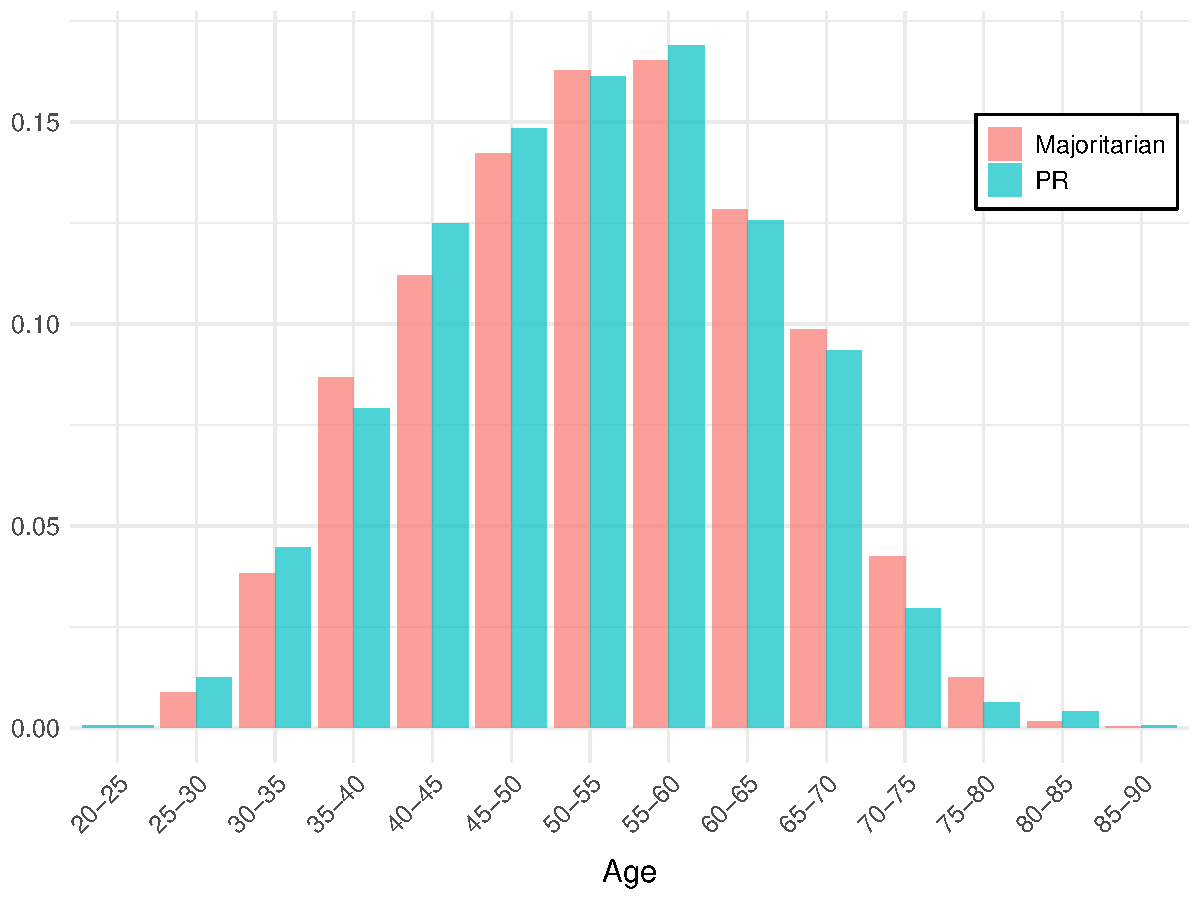
\includegraphics[width = 0.9\textwidth]{../figure/paper/age_smd_vs_pr_winners.pdf}
	\caption{Age Composition of Legislators Elected from the Two Tiers}
	\label{fig:pr_vs_smd}
\end{figure}



\begin{figure}[!htbp]
	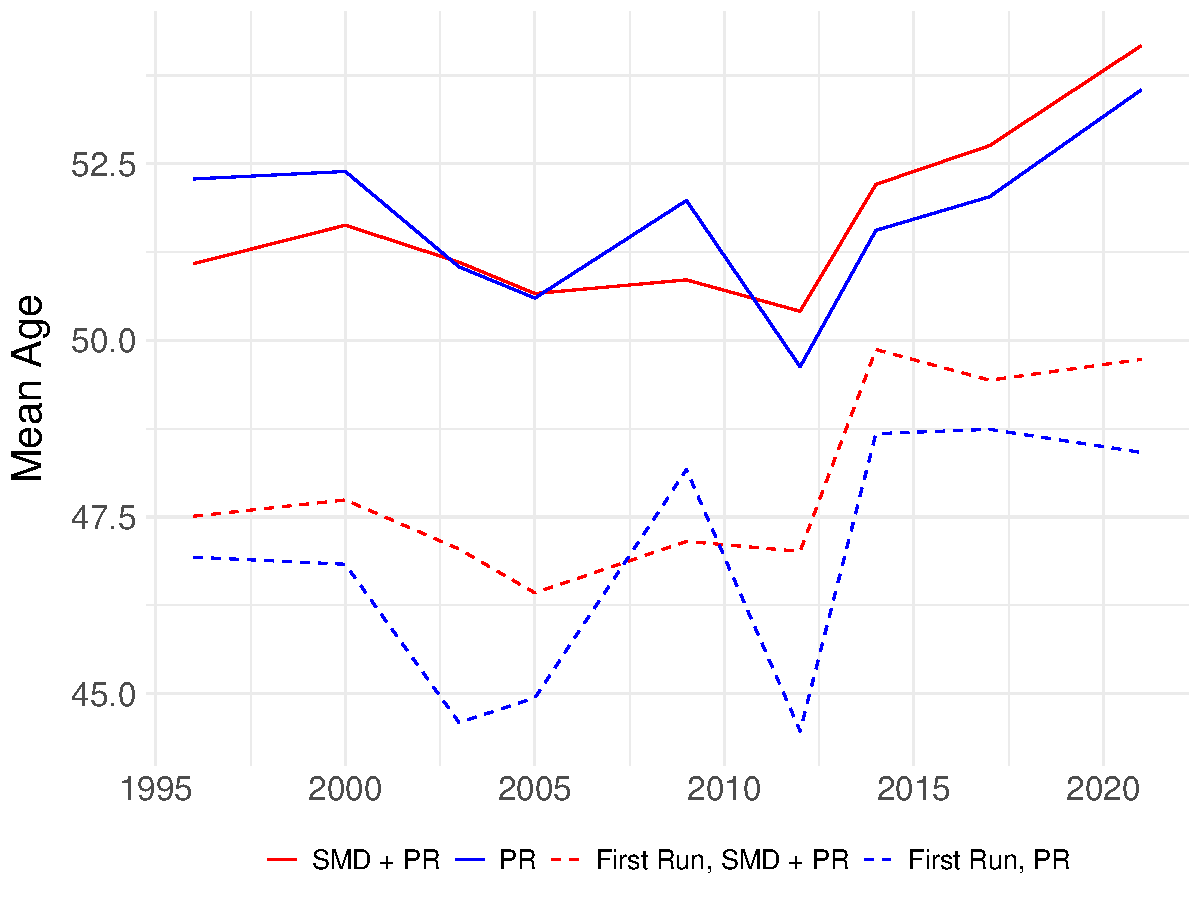
\includegraphics[width = 0.9\textwidth]{../figure/paper/age_first_run.pdf}
	\caption{Age Comparison: Average vs. New Candidates}
	\label{fig:ageFirstRun}
\end{figure}



\section{Conclusion}

% TODO: write

\newpage

\bibliography{../bibliography.bib}
\bibliographystyle{apalike}

\newpage

\appendix

\setcounter{table}{0}
\setcounter{figure}{0}
\renewcommand{\thetable}{A\arabic{table}}
\renewcommand{\thefigure}{A\arabic{figure}}

\section{Summary Statistics}

\subsection{Candidate-Level Summary Statistics}

% TODO: add a revised table
\begin{table}[!htbp] \centering \renewcommand*{\arraystretch}{1.1}\caption{Summary Statistics}\resizebox{\textwidth}{!}{
\begin{threeparttable}
\begin{tabular}{l|cccccccc}
\toprule
Variable & N & Mean / \% & Std. Dev. & Min & \% 25 & \% 50 & \% 75 & Max \\ 
\midrule
Gender & 6935 &  &  &  &  &  &  &  \\ 
... Female & 881 & 12.7\% &  &  &  &  &  &  \\ 
... Male & 6054 & 87.3\% &  &  &  &  &  &  \\ 
N of wins before & 6935 & 1.776 & 2.487 & 0 & 0 & 1 & 3 & 19 \\ 
Incumbency & 6935 &  &  &  &  &  &  &  \\ 
... Incumbent & 3129 & 45.1\% &  &  &  &  &  &  \\ 
... Non-Incumbent & 3806 & 54.9\% &  &  &  &  &  &  \\ 
List Rank & 6935 & 4.317 & 6.976 & 1 & 1 & 2 & 4 & 52\\ 
Dual Listing & 6935 &  &  &  &  &  &  &  \\ 
... Yes & 5292 & 76.3\% &  &  &  &  &  &  \\ 
... No & 1643 & 23.7\% &  &  &  &  &  &  \\ 
\bottomrule
\end{tabular}
\begin{tablenotes}[flushleft]
  \scriptsize{
    \item Candidate-level summary statistics. 
    \item \textit{Data source}: \citet{reedsmith2018} 
  }
\end{tablenotes}
\end{threeparttable}
}
\label{tab:stats}
\end{table}



\newpage

\subsection{Magnitudes of PR Blocks, 1996 - 2021}

% created manually
\begin{table}[!htbp]
\begin{threeparttable}
\begin{tabular}{lccccccccc}
\toprule
Bloc & 1996 & 2000 & 2003 & 2005 & 2009 & 2012 & 2014 & 2017 & 2021 \\
\midrule
Hokkaido & 9 & 8 & 8 & 8 & 8 & 8 & 8 & 8 & 8 \\
Tohoku & 16 & 14 & 14 & 14 & 14 & 14 & 14 & 13 & 13 \\
Kita-kanto & 21 & 20 & 20 & 20 & 20 & 20 & 20 & 19 & 19 \\
Tokyo & 19 & 17 & 17 & 17 & 17 & 17 & 17 & 17 & 17 \\
Minami-kanto & 23 & 21 & 22 & 22 & 22 & 22 & 22 & 22 & 22 \\
Hokuriku Shinetsu & 13 & 11 & 11 & 11 & 11 & 11 & 11 & 11 & 11 \\
Tokai & 23 & 21 & 21 & 21 & 21 & 21 & 21 & 21 & 21 \\
Kinki & 33 & 30 & 30 & 30 & 29 & 29 & 29 & 28 & 28 \\
Chugoku & 13 & 11 & 11 & 11 & 11 & 11 & 11 & 11 & 11 \\
Shikoku & 7 & 6 & 6 & 6 & 6 & 6 & 6 & 6 & 6 \\
Kyushu & 23 & 21 & 21 & 21 & 21 & 21 & 21 & 20 & 20 \\
\bottomrule
\end{tabular}
\begin{tablenotes}[flushleft]
  \scriptsize{
    \item Magnitudes of each PR regional district for elections 1996 - 2021. 
    \item \textit{Data source}: \citet{reedReedSmithJapaneseHouse2017, ministryofinternalaffairsandcommunicationsElectionSenkyo2024}
  }
\end{tablenotes}
\end{threeparttable}
\caption{Magnitudes of PR Blocks}
\label{tab:distM}
\end{table}

\newpage

\subsection{Distribution of List Rank}

\begin{figure}[!htbp]
	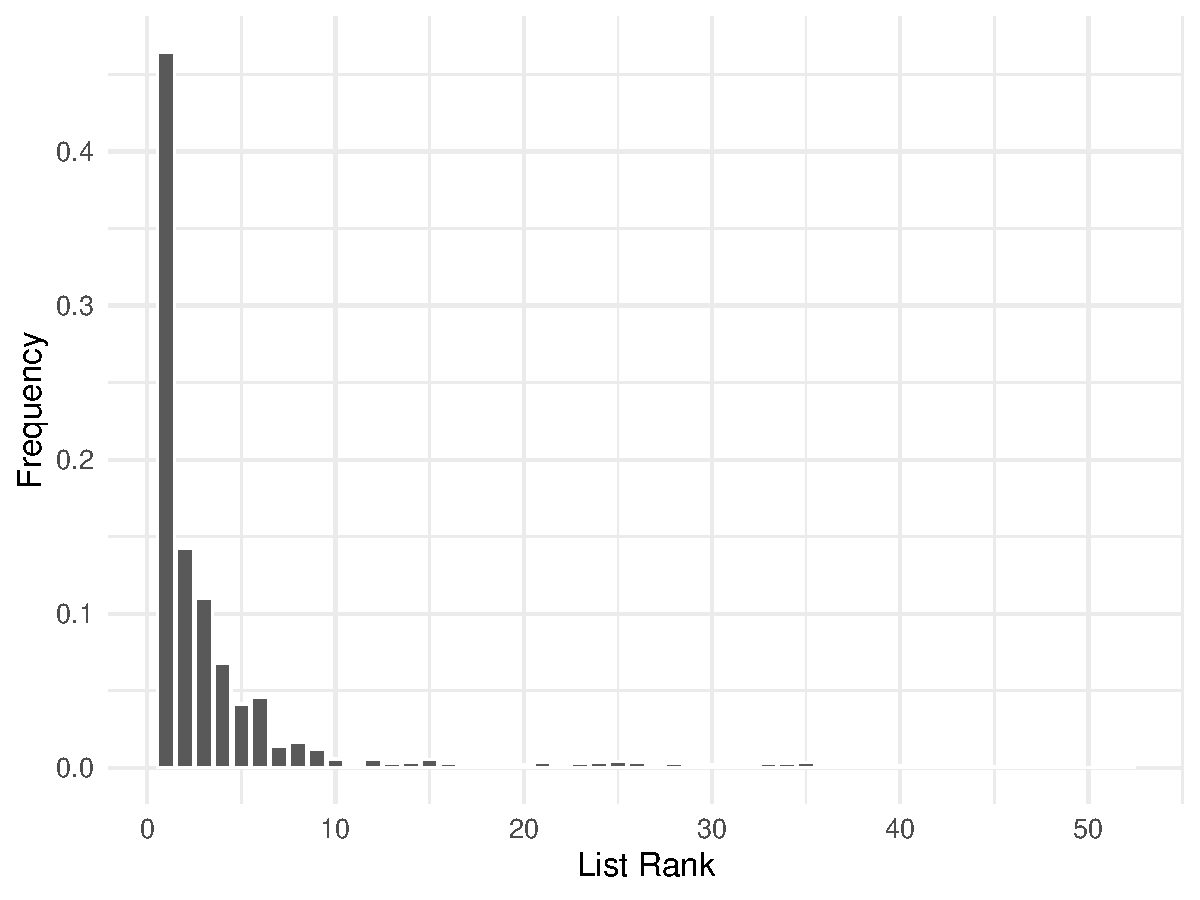
\includegraphics[width = 0.9\textwidth]{../figure/paper/pr_rank_distribution.pdf}
	\caption{Distribution of List Rank}
	\label{fig:distRank}
\end{figure}

\newpage

\subsection{Age of Winners}

\begin{figure}[!htbp]
	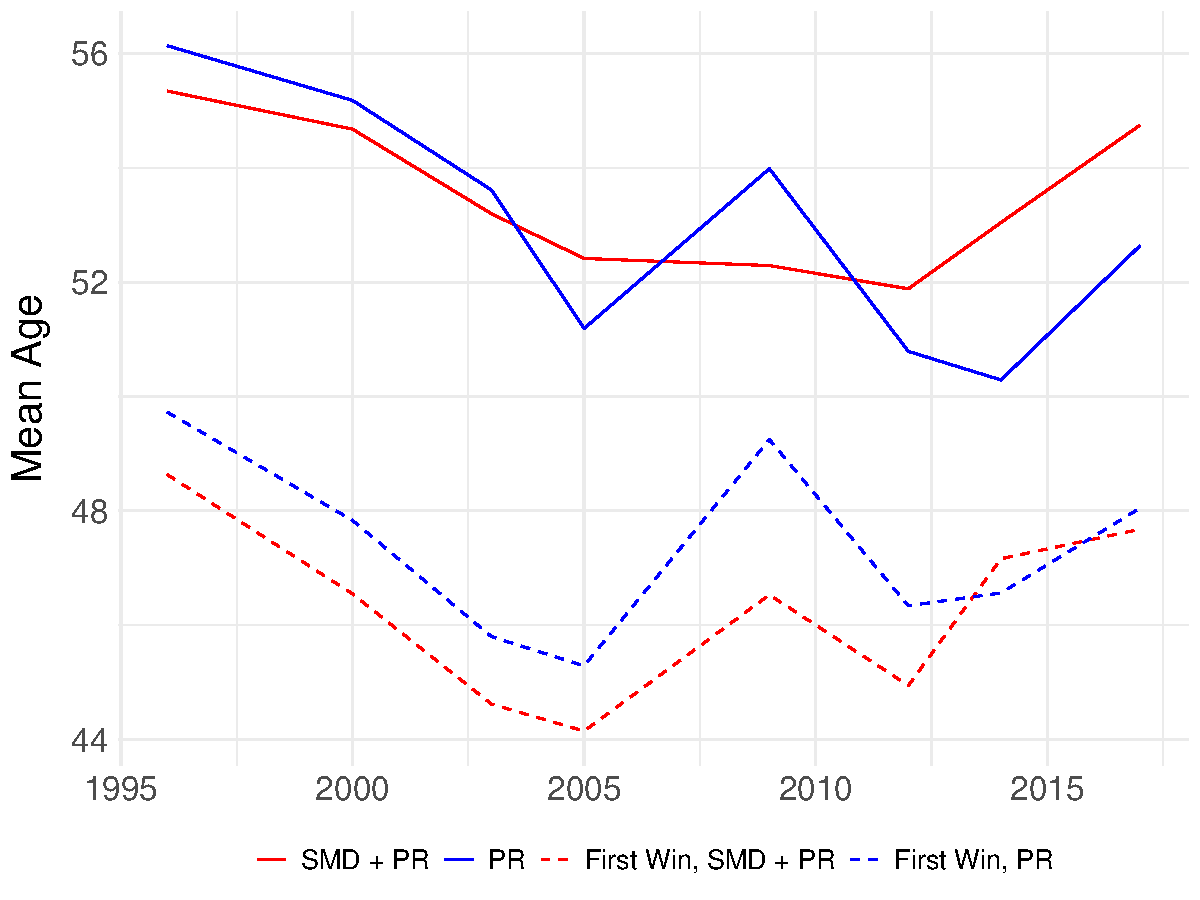
\includegraphics[width = 0.9\textwidth]{../figure/paper/age_first_win.pdf}
	\caption{Age Comparison: Average vs. New Legislators}
	\label{fig:ageFirstWin}
\end{figure}	

\newpage

\section{Additional Analyses}

\subsection{Party-level Analysis}

\subsubsection*{Komeito}


\begin{table}
\begin{center}
\begin{tabular}{l c c c c c c c c c c}
\hline
 & \multicolumn{4}{c}{List Rank} & \multicolumn{3}{c}{Dual Listing} & \multicolumn{3}{c}{Dual Listing (Tie)} \\
\cline{2-5} \cline{6-8} \cline{9-11}
 & Model 1 & Model 2 & Model 3 & Model 4 & Model 5 & Model 6 & Model 7 & Model 8 & Model 9 & Model 10 \\
\hline
Total Wins       & $-0.21^{***}$ &               &           & $-0.12^{***}$ & $0.32$   &          & $0.12$   & $0.34$   &          & $0.38$   \\
                 & $(0.02)$      &               &           & $(0.03)$      & $(0.19)$ &          & $(0.27)$ & $(0.24)$ &          & $(0.34)$ \\
Incumbency       &               & $-0.79^{***}$ &           & $-0.46^{***}$ &          & $1.50$   & $1.21$   &          & $1.17$   & $0.35$   \\
                 &               & $(0.07)$      &           & $(0.12)$      &          & $(0.88)$ & $(1.15)$ &          & $(1.25)$ & $(1.70)$ \\
Dual Listing     &               &               & $-0.26$   & $0.20$        &          &          &          &          &          &          \\
                 &               &               & $(0.23)$  & $(0.30)$      &          &          &          &          &          &          \\
Tie              &               &               &           & $-1.63$       &          &          &          &          &          &          \\
                 &               &               &           & $(1.96)$      &          &          &          &          &          &          \\
Female           &               &               &           & $-0.13$       &          &          & $-0.49$  &          &          & $1.06$   \\
                 &               &               &           & $(0.10)$      &          &          & $(1.19)$ &          &          & $(1.45)$ \\
Block Magnitude  &               &               &           & $0.04^{***}$  &          &          & $-0.06$  &          &          & $-0.05$  \\
                 &               &               &           & $(0.01)$      &          &          & $(0.06)$ &          &          & $(0.10)$ \\
Total Wins x Tie &               &               &           & $0.64$        &          &          &          &          &          &          \\
                 &               &               &           & $(0.71)$      &          &          &          &          &          &          \\
\hline
Year FE          & Yes           & Yes           & Yes       & Yes           & Yes      & Yes      & Yes      & Yes      & Yes      & Yes      \\
Party FE         & No            & No            & No        & No            & No       & No       & No       & No       & No       & No       \\
AIC              & $18.00$       & $1134.87$     & $1264.37$ & $1042.07$     & $57.30$  & $56.69$  & $61.28$  & $38.40$  & $39.19$  & $43.55$  \\
BIC              & $52.05$       & $1168.92$     & $1298.42$ & $1098.83$     & $87.57$  & $86.96$  & $102.91$ & $68.67$  & $69.46$  & $85.18$  \\
Log Likelihood   & $0.00$        & $-558.43$     & $-623.18$ & $-506.04$     & $-20.65$ & $-20.35$ & $-19.64$ & $-11.20$ & $-11.59$ & $-10.78$ \\
Deviance         & $180.36$      & $195.93$      & $309.02$  & $91.14$       & $41.30$  & $40.69$  & $39.28$  & $22.40$  & $23.19$  & $21.55$  \\
Num. obs.        & $325$         & $325$         & $325$     & $325$         & $325$    & $325$    & $325$    & $325$    & $325$    & $325$    \\
\hline
\multicolumn{11}{l}{\scriptsize{\item $^{***}p<0.001$; $^{**}p<0.01$; $^{*}p<0.05$. Standard errors in parentheses.
\item Dependent variable: candidate $i$'s list rank (columns 1-4) dual listing status (columns 5-7), and whether the candidate has a tie on the list (columns 8-10).
\item Estimated models: negatige binomial (columns 1-4) and logit (columns 5-10).}}
\end{tabular}
\caption{Regression Results for Komeito Candidates}
\label{tab:komeito}
\end{center}
\end{table}


\newpage

\subsubsection*{JCP}


\begin{table}[!htbp]
\begin{center}
\scalebox{0.7}{
\begin{threeparttable}
\begin{tabular}{l D{.}{.}{4.5} D{.}{.}{4.5} D{.}{.}{4.3} D{.}{.}{4.5} D{.}{.}{4.3} D{.}{.}{4.3} D{.}{.}{4.5} D{.}{.}{3.3} D{.}{.}{5.3} D{.}{.}{5.5}}
\toprule
 & \multicolumn{4}{c}{List Rank} & \multicolumn{3}{c}{Dual Listing} & \multicolumn{3}{c}{Dual Listing (Tie)} \\
\cmidrule(lr){2-5} \cmidrule(lr){6-8} \cmidrule(lr){9-11}
 & \multicolumn{1}{c}{Model 1} & \multicolumn{1}{c}{Model 2} & \multicolumn{1}{c}{Model 3} & \multicolumn{1}{c}{Model 4} & \multicolumn{1}{c}{Model 5} & \multicolumn{1}{c}{Model 6} & \multicolumn{1}{c}{Model 7} & \multicolumn{1}{c}{Model 8} & \multicolumn{1}{c}{Model 9} & \multicolumn{1}{c}{Model 10} \\
\midrule
Total Wins       & -0.22^{***}             &                         &                         & -0.10^{***}             & -0.03                   &                         & -0.04                   & -2.19^{*}               &                         & -1.40                   \\
                 & (0.02)                  &                         &                         & (0.03)                  & (0.05)                  &                         & (0.08)                  & (0.98)                  &                         & (1.13)                  \\
Incumbency       &                         & -0.95^{***}             &                         & -0.72^{***}             &                         & -0.12                   & -0.17                   &                         & -19.85                  & -17.22                  \\
                 &                         & (0.08)                  &                         & (0.11)                  &                         & (0.23)                  & (0.34)                  &                         & (2367.75)               & (2043.44)               \\
Dual Listing     &                         &                         & 0.07                    & -0.06                   &                         &                         &                         &                         &                         &                         \\
                 &                         &                         & (0.06)                  & (0.06)                  &                         &                         &                         &                         &                         &                         \\
Tie              &                         &                         &                         & -0.03                   &                         &                         &                         &                         &                         &                         \\
                 &                         &                         &                         & (0.11)                  &                         &                         &                         &                         &                         &                         \\
Female           &                         &                         &                         & 0.04                    &                         &                         & -0.12                   &                         &                         & -0.99^{*}               \\
                 &                         &                         &                         & (0.05)                  &                         &                         & (0.21)                  &                         &                         & (0.46)                  \\
Block Magnitude  &                         &                         &                         & 0.05^{***}              &                         &                         & 0.07^{***}              &                         &                         & 0.13^{***}              \\
                 &                         &                         &                         & (0.00)                  &                         &                         & (0.01)                  &                         &                         & (0.04)                  \\
Total Wins x Tie &                         &                         &                         & 0.29                    &                         &                         &                         &                         &                         &                         \\
                 &                         &                         &                         & (0.51)                  &                         &                         &                         &                         &                         &                         \\
\midrule
Year FE          & \multicolumn{1}{c}{Yes} & \multicolumn{1}{c}{Yes} & \multicolumn{1}{c}{Yes} & \multicolumn{1}{c}{Yes} & \multicolumn{1}{c}{Yes} & \multicolumn{1}{c}{Yes} & \multicolumn{1}{c}{Yes} & \multicolumn{1}{c}{Yes} & \multicolumn{1}{c}{Yes} & \multicolumn{1}{c}{Yes} \\
Party FE         & \multicolumn{1}{c}{No}  & \multicolumn{1}{c}{No}  & \multicolumn{1}{c}{No}  & \multicolumn{1}{c}{No}  & \multicolumn{1}{c}{No}  & \multicolumn{1}{c}{No}  & \multicolumn{1}{c}{No}  & \multicolumn{1}{c}{No}  & \multicolumn{1}{c}{No}  & \multicolumn{1}{c}{No}  \\
AIC              & 1775.10                 & 1750.64                 & 1897.57                 & 1568.00                 & 628.43                  & 628.60                  & 610.54                  & 178.03                  & 180.35                  & 162.47                  \\
BIC              & 1820.69                 & 1796.23                 & 1943.16                 & 1638.45                 & 669.87                  & 670.04                  & 664.42                  & 219.48                  & 221.79                  & 216.34                  \\
Log Likelihood   & -876.55                 & -864.32                 & -937.78                 & -767.00                 & -304.21                 & -304.30                 & -292.27                 & -79.02                  & -80.18                  & -68.23                  \\
Deviance         & 385.60                  & 372.88                  & 423.51                  & 191.69                  & 608.43                  & 608.60                  & 584.54                  & 158.03                  & 160.35                  & 136.47                  \\
Num. obs.        & 466                     & 466                     & 466                     & 466                     & 466                     & 466                     & 466                     & 466                     & 466                     & 466                     \\
\bottomrule
\end{tabular}
\begin{tablenotes}[flushleft]
\scriptsize{\item $^{***}p<0.001$; $^{**}p<0.01$; $^{*}p<0.05$. Standard errors in parentheses.
\item Dependent variable: candidate $i$'s list rank (columns 1-4) dual listing status (columns 5-7), and whether the candidate has a tie on the list (columns 8-10).
\item Estimated models: negatige binomial (columns 1-4) and logit (columns 5-10).}
\end{tablenotes}
\end{threeparttable}
}
\caption{Regression Results for JCP Candidates}
\label{tab:jcp}
\end{center}
\end{table}


\end{document}































